\chapter{Relativity}

\textit{Imagination is more important than knowledge. Knowledge is limited. Imagination encircles the world.}\\
\noindent\textbf{-   Albert Einstein}

\vspace{0.5cm}

\begin{marginfigure}%
  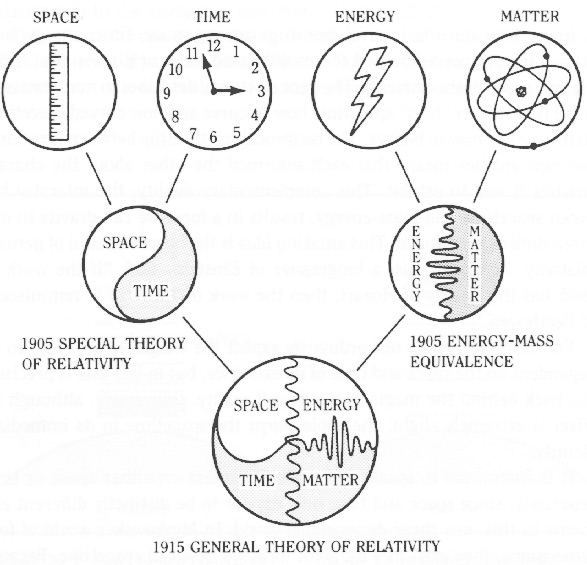
\includegraphics[width=\linewidth]{space_time_energy.jpg}
  \caption{Special and general relativity}
  \label{fig:marginfig}
\end{marginfigure}

The theory of relativity usually encompasses two theories by Albert Einstein: special relativity and general relativity.  Concepts introduced by the theories of relativity include spacetime as a unified entity of space and time, relativity of simultaneity, kinematic and gravitational time dilation, and length contraction.

\section{Galilean-Newtonian Relativity}
\begin{marginfigure}[0pt]
  
\includegraphics[width=\linewidth]{mboat.jpg}
  \caption{Galilean boat}
  \label{fig:marginfig}
\end{marginfigure}
Galilean invariance, Galilean relativity or Newtonian relativity states Newtonian physics operates the same in all inertial (non-accelerating) frames. Galileo Galilei first described this principle in 1632 in his \textit{Dialogue Concerning the Two Chief World Systems}.  He describes a ship traveling at constant velocity, without rocking, on a smooth sea.  In this ship any observer doing experiments below the deck would not be able to tell whether the ship was moving or stationary.\\
Unfortunately Galilean invariance did not agree with Maxwell's equations describing electromagnetism.  The first problem is that electromagnetic theory describes electromagnetic waves, namely light, moving at a constant speed no matter the velocity of the frame of reference.  In addition all experiments show light moving at a constant speed.  The second problem with electromagnetic theory is that electromagnetic forces seem to be dependent on the velocity of the frame of reference.  Namely, in a frame moving with a charged particle there are no magnetic forces however the same particle observed from a frame in which it is moving could see magnetic forces.  Forces, however, should not be dependent on the velocity of the frame of reference. 

\marginnote[-150pt]{
\subsection{Galilean Transformation}
$x$ transforms to $x'$ in a frame moving in the x-direction at speed $v$.
$$\overrightarrow{v}=v\hat{x}$$
$$x'= x-vt \hspace{2cm} y'=y$$
$$z'= z \hspace{2cm} t'=t$$
$$\overrightarrow{u}'=\overrightarrow{u}-\overrightarrow{v}$$
$$\overrightarrow{E}'=\overrightarrow{E}-\overrightarrow{v}\times\overrightarrow{B}$$
$$\overrightarrow{B}'=\overrightarrow{B}+\frac{1}{c^2}\overrightarrow{v}\times\overrightarrow{E}$$
}


\section{Einstein's Relativity}
Einstein's relativity dictates the laws of mechanics, including electromagnetism, must be the same in all inertial frames and that the speed of light is constant. 

\section{Time Dilation}
\begin{marginfigure}%
  
\includegraphics[width=\linewidth]{slow_clock.jpg}
  \caption{Moving clocks run slowly}
  \label{fig:marginfig}
\end{marginfigure}
Consider a light clock which consists of a light source next to a photocell opposite a mirror.  They are a distance $D$ apart.  Light travels at speed $c$ and travels a distance $2D$.  The time it takes is $\Delta \tau$
$$\Delta \tau=\frac{2D}{c}$$
Now consider the light clock moving perpendicular to the length $D$ at a speed $v$.  In this frame the light takes a longer path but still travels at speed $c$.  The time for the light to travel in this frame is $\Delta t'$.
$$\Delta t=\frac{2\sqrt{D^2+(\nicefrac{v \Delta t}{2})^2}}{c}$$
Squaring each side of both equations.
$$(\Delta \tau)^2=\frac{4D^2}{c^2} \hspace{1cm} (\Delta t)^2=\frac{4D^2+v^2(\Delta t)^2}{c^2}$$
\marginnote[-100pt]{$\Delta \tau $ is the proper time interval.  This is defined as the time separating two events that take place at the same point in space. }
Combining these equations and solving for $\Delta t$ yields the following.
$$\Delta t=\frac{\Delta \tau}{\sqrt{1-\frac{v^2}{c^2}}}=\gamma \Delta \tau $$
Note the factor $\nicefrac{1}{\sqrt{1-\nicefrac{v^2}{c^2}}}$ is always greater than one, $\gamma>1$.  Therefore   $\Delta t > \Delta \tau$.  The clock tics more slowly when it is observed moving.
\begin{figure}%
  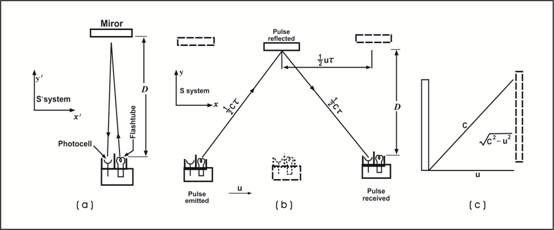
\includegraphics[width=\linewidth]{time_dilation.jpg}
  \caption{Time dilation}
  \label{fig:marginfig}
\end{figure}


\section{Length Contraction}

\begin{marginfigure}[180pt]
  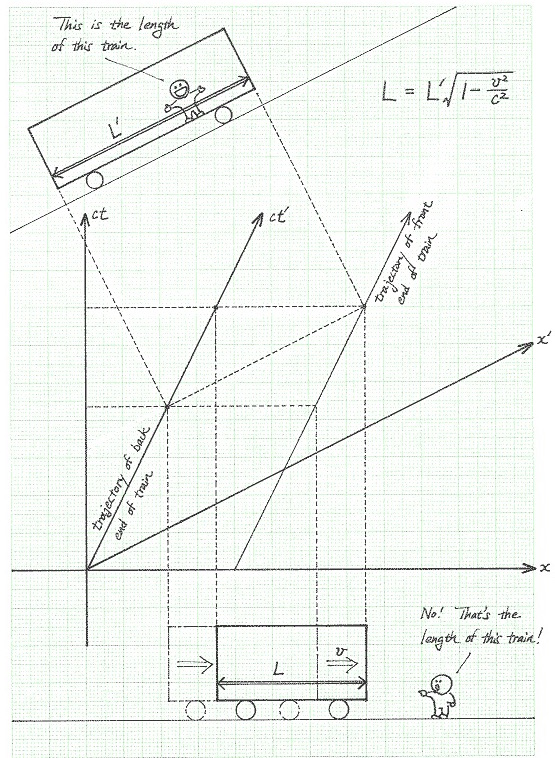
\includegraphics[width=\linewidth]{LorentzContraction.jpg}
  \caption{Length contraction}
  \label{fig:marginfig}
\end{marginfigure}
Now consider measuring the velocity of an object.  This always requires retrieving information from each frame of reference.  One could view a moving clock and measure the distance it moved between flashes.  The time measurement would be in the moving frame $\Delta t$ while the length measurement would be in the rest frame $L$.  
$$v=\frac{L}{\Delta t}$$
Alternately the velocity could be determined using a still clock with proper time interval $\Delta \tau$ and an object whose length is measured while moving $l$.
$$v=\frac{l}{\Delta \tau}$$
Equating the velocities gives the following.
$$\frac{L}{\Delta t}=\frac{l}{\Delta \tau}$$
Expressing $\Delta \tau$ in terms of $\Delta t$ gives an expression for $L$ in terms of $l$.
$$\frac{L}{	\gamma \Delta \tau}=\frac{l}{\Delta \tau}$$
$$L=\gamma l=\frac{l}{\sqrt{1-\frac{v^2}{c^2}}}$$
This means the moving length $l$ is shorter than the proper length $L$.  This is known as length contraction.  Moving objects appear squished.
\marginnote[-100pt]{$L$ is the proper length.  The proper length or rest length refers to the length of an object in the object's rest frame. }


\section{Lorentz Transformation}
\begin{marginfigure}[50pt]
  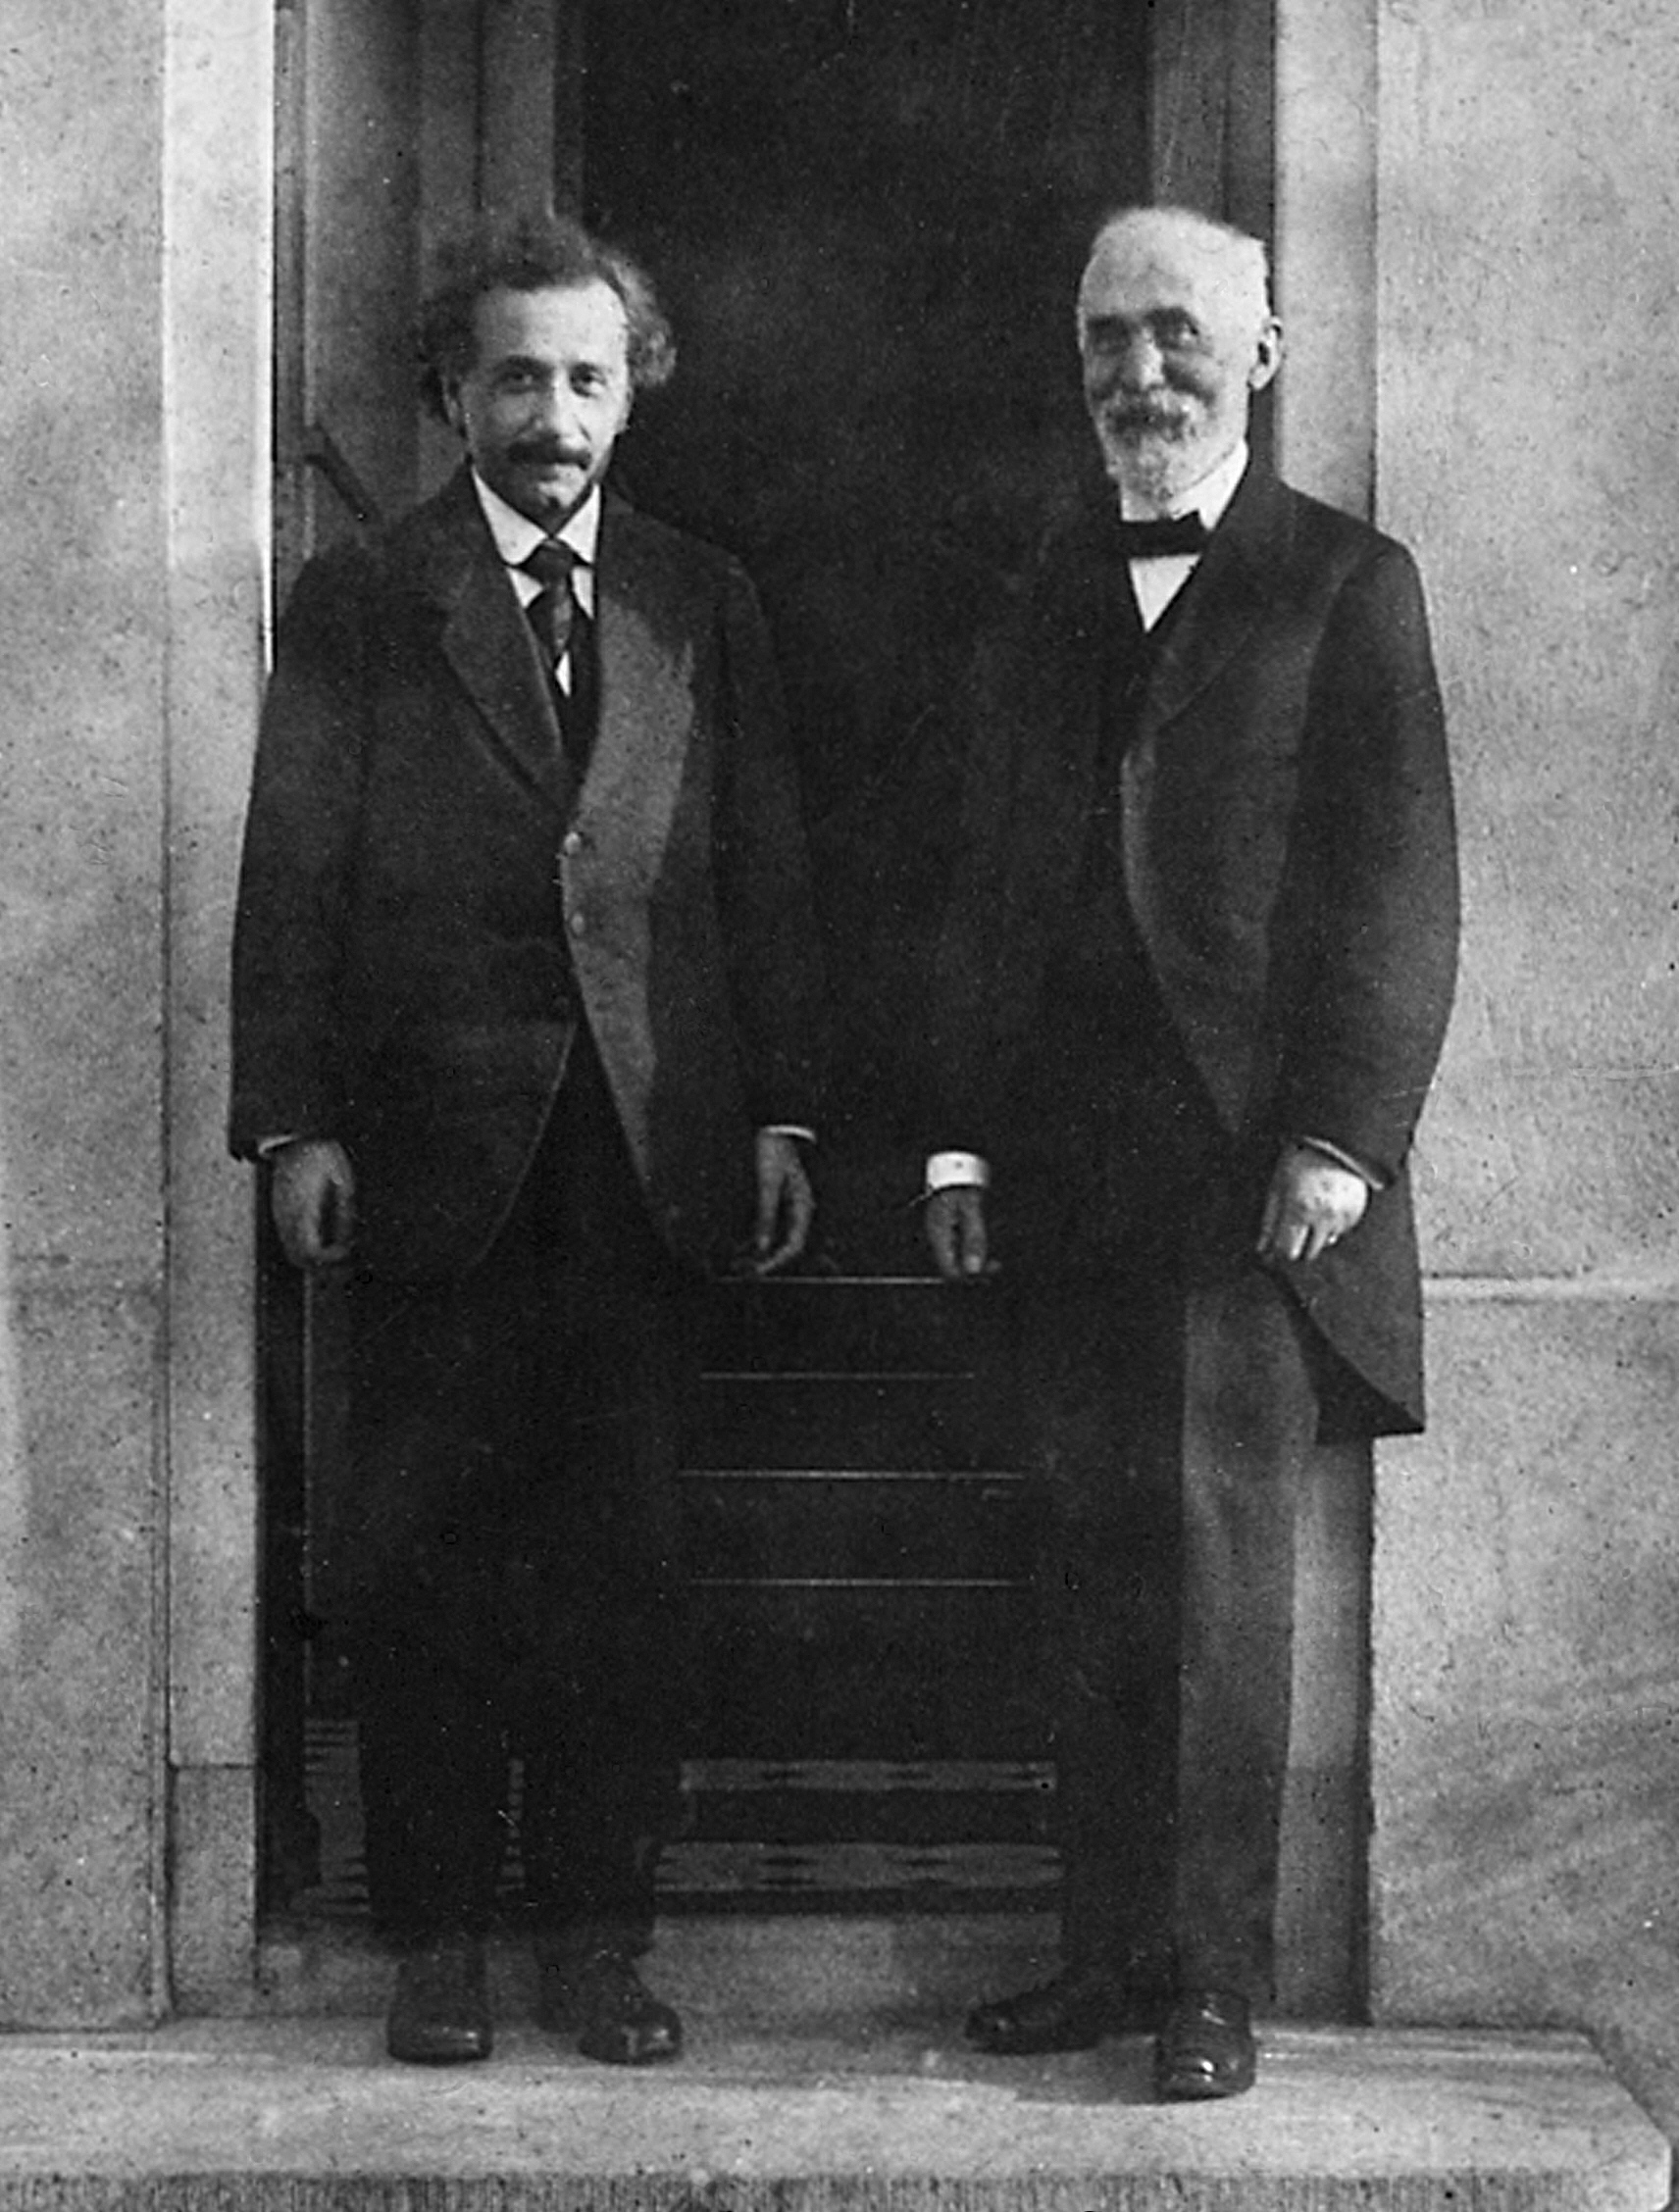
\includegraphics[width=\linewidth]{Einstein_Lorentz.jpg}
  \caption{Albert Einstein and Hendrik Lorentz \#biffles4life}
  \label{fig:marginfig}
\end{marginfigure}

The Lorentz transformation is a coordinate transformation between two coordinate frames that move at constant velocity relative to each other.  Here $x$ is transformed to $x'$ by taking measurements in a frame moving at $\overrightarrow{v}=v\hat{x}$.  $$x'= \gamma(x-vt)$$ 
The $y$ and $z$ coordinates are left invariant in this transformation.  
$$ y'=y \hspace{2cm}z'= z$$
Time is transformed in the moving frame as follows.
$$ \hspace{2cm} t'=\gamma \left( t -\frac{v}{c^2}x\right)$$
The velocity of an object in the rest frame is measured as $\overrightarrow{u}$.  The x-component of the velocity is transformed as follows.
$$u_x'=\frac{u_x-v}{1-\frac{u_xv}{c^2}}$$

\section{Relativistic Mechanics}
Special relativity gives new definitions to momentum and kinetic energy.
$$\overrightarrow{p}=m \overrightarrow{v}=\gamma m_0 \overrightarrow{v}$$
\marginnote[-20pt]{An interpretation relativistic momentum uses the concept of relativistic mass.  At high velocity the mass transforms from the rest mass $m_0$ to $m$.
$$m=\gamma m_0$$}
Once relativistic momentum is defined the relativistic force may be derived using Newton's second law.
$$\overrightarrow{F}_{net}=\frac{d\overrightarrow{p}}{dt}$$
Once the relativistic force is defined the relativistic kinetic energy may be derived using work-energy theorem.
$$\Delta KE=W_{net}= \int \overrightarrow{F}_{net}\cdot d\overrightarrow{r}$$
This yields the following expression for relativistic kinetic energy.
$$KE=\gamma m_0c^2-m_0c^2= m c^2-m_0c^2$$
The kinetic energy is the difference between two terms.  The first term $E$ changes with velocity.  The second term, know as the rest energy $E_0$ is independent of velocity.
$$KE=E-E_0$$
The total energy $E$ is defined as the sum of the kinetic energy and the rest energy.
$$E=KE+E_0$$
The total energy and rest energy are written as follows.
$$E=\gamma mc^2$$
\marginnote[0pt]{$$E^2=p^2c^2+(mc^2)^2$$}
$$E_0=m_0c^2$$
This expression for the rest energy describes a relationship between energy and mass.  This is known as mass-energy equivalence.

\section{General Relativity}
\begin{marginfigure}[0pt]
  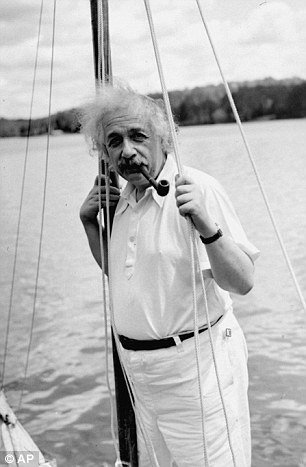
\includegraphics[width=\linewidth]{EinsteinBoat.jpg}
  \caption{Einstein on a boat!}
  \label{fig:marginfig}
\end{marginfigure}
General relativity describes the effect of gravity on spacetime.  Mass is an inertial quantity.  Newton's second law relates to inertial mass.  
$$F_{net}=m_{i}a$$ 
Gravity is different than the other forces in nature because mass gives rise to its field interaction.
$$F_g=m_gg$$.  
Therefore the strength of the gravitational field $g$ is equal to the acceleration $a$.  The equivalence principle states that a gravitational field is indistinguishable from acceleration.  This gives the theory the ability to analyze the behavior of time, space and light in proximity to mass.\\
The net time dilation in a spherically symmetric gravitational field can is considered. It is written below.
$$\Delta t=\frac{\Delta \tau}{\sqrt{1-\frac{2GM}{rc^2}}}=\frac{\Delta \tau}{\sqrt{1-\frac{v_e^2}{c^2}}}$$
\begin{marginfigure}[-60pt]
  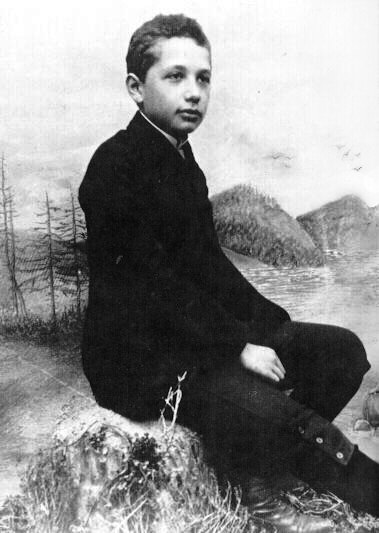
\includegraphics[width=\linewidth]{Einstein14.jpg}
  \caption{Albert Einstein at 14}
  \label{fig:marginfig}
\end{marginfigure}
The proper time is outside the gravitational field, out at $r=\infty$.  Note that this is simply special relativity applied when the object is moving at the escape velocity from the field.
Other effects include bending of light and curvature of space.
